\documentclass[10pt,a4paper]{beamer}
\usepackage[utf8]{inputenc}
\usepackage[english]{babel}
\usepackage{amsmath}
\usepackage{amsfonts}
\usepackage{amssymb}
\usepackage[ND,SEQ]{../prftree}
\usepackage{mathrsfs}
\usepackage{graphicx}


\author{Paolo Comensoli}
\usetheme{Malmoe}
\title{Hyper-resolution applications}
\date{March 15, 2019}

\newcommand{\textbl}[1]{\textbf{\textcolor{blue}{#1}}}
\newcommand{\pausa}{} %secondo argomento vuoto per non avere le transizioni, altrimenti inserire \pause

\newcommand{\E}{\mathscr{E}}
\newcommand{\D}{\mathscr{D}}
\newcommand{\K}{\mathbb{K}}



%\newcommand*{\QEDF}{\hfill\ensuremath{\blacksquare}}
\newcommand*{\QED}{\hfill\ensuremath{\square}}
\newcommand*{\QEDn}{\newline\hspace*{1cm}\QED} %quadratino nella lina sottostante


\newcommand*\npred{\,\includegraphics[scale=0.023]{../simboli/not-predecessor.eps}\,}
\newcommand*\pred{\,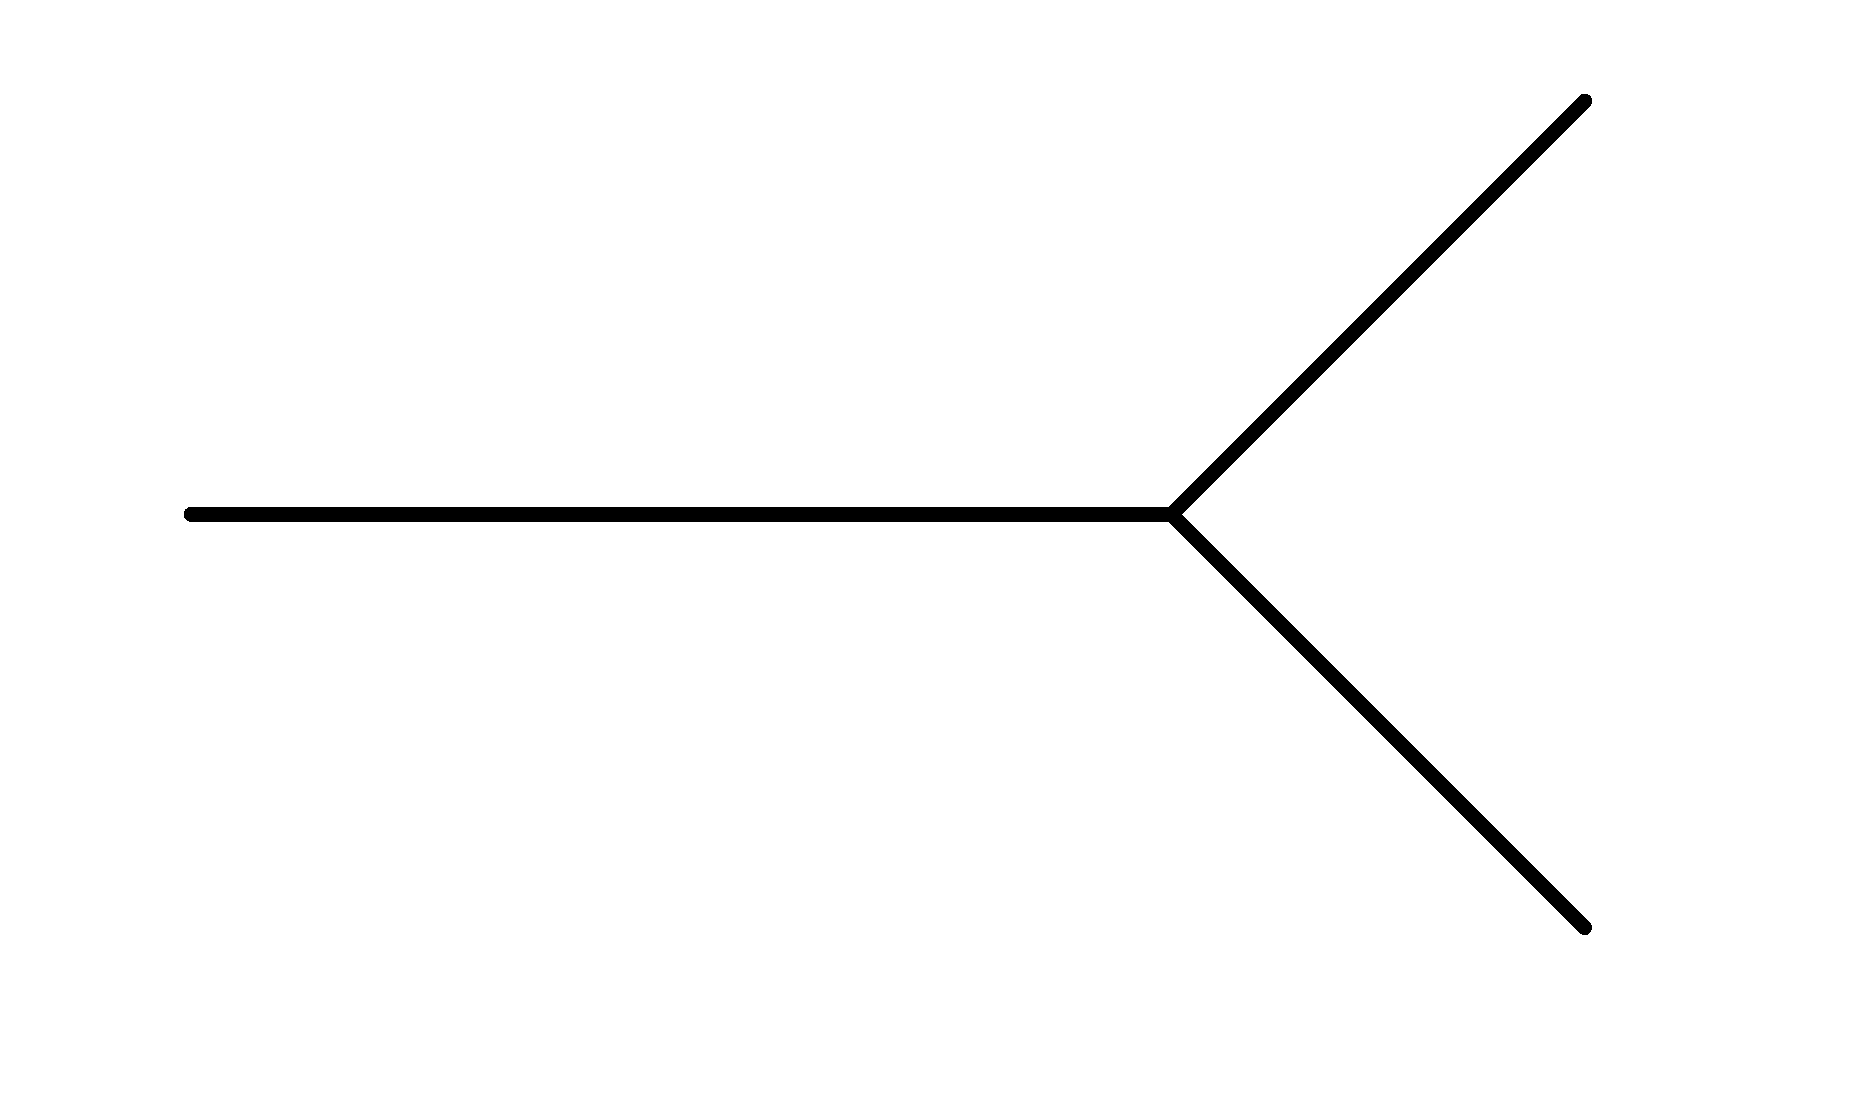
\includegraphics[scale=0.023]{../simboli/predecessor.eps}\,}



\let\oldemptyset\emptyset
\let\emptyset\varnothing
\let\o\vee
\let\e\wedge
\let\bottom\perp


%\newtheorem{proposition}[theorem]{Proposition}
%\newtheorem{definition}[theorem]{Definition}
%\newtheorem{lemma}[theorem]{Lemma}
%\newtheorem{corollary}[theorem]{Corollary}
%\newtheorem*{example}{Example}
\newtheorem*{conjecture}{Conjecture}

\begin{document}
\frame{\maketitle}

\section{The hyper-resolution principle}
\frame{
\frametitle{Introduction}
\begin{itemize}
\item In 1965, J.A. Robinson published "\textbl{A Machine-oriented logic} based on the resolution principle."
\item A single inference principle that provides a \textbl{complete system} of propositional calculus. \
\item In 1972, Matijasevi\v{c} published "Application of the methods of the theory of logical derivation to \textbl{graph theory}." 
\item In 1980 Vladimir Lifschitz published "Semantical completeness theorems in logic and \textbl{algebra}."
\end{itemize}}

\frame{
\frametitle{Preliminaries:}
\begin{itemize}
\item \textbl{Atomic formulae:} a formula that contains no logical connectors. 
\item \textbl{Literal:} is either an atomic formula, or has the form $\neg A$ where $\neg$ is the negation symbol and $A$ is an atomic formula. Literals will be denoted using Latin capital letters $A,B,C,...$. 
\item \textbl{Clause:} is a finite set of literals. Clauses are denoted by Greek capital letters $\Gamma,\Sigma ,\Pi, \Delta...$. The singleton $\{A\}$ is denoted by its element $A$.
\item A set $S$ of clause is \textbl{satisfiable} if there is a model of $S$; otherwise $S$ is \textbl{unsatisfiable}
\end{itemize}
}

\frame{
\begin{definition}
%Let $\Gamma_1$ and $\Gamma_2$ be two clauses, let $P$ be a literal such that $P\in\Gamma_1\,$ and $\neg P\in\Gamma_2$; then $\Pi =\Gamma_1\cup\Gamma_2\setminus\{P,\neg P\}$ is called the \textbl{resolvent} of $\Gamma_1$ and\nobreak$\,\Gamma_2$.
\begin{itemize}
\item  $\Gamma_1$ and $\Gamma_2$: clauses
\item  $P\in\Gamma_1\,$ and $\neg P\in\Gamma_2$
\item  $\Pi =\Gamma_1\cup\Gamma_2\setminus\{P,\neg P\}$ is called the \textbl{resolvent} of $\Gamma_1$ and\nobreak$\,\Gamma_2$
\end{itemize}
\end{definition}

The {\textbl{resolution principle}}:\\
\textit{If $\Pi$ is unsatisfiable and is the resolvent of  $\Gamma_1$ and $\Gamma_2$; then  $\Gamma_1$ and $\Gamma_2$ are unsatisfiable.}

\begin{example}
\begin{center}
\begin{tabular}{ccc}
$\prftree{A}{\neg A}{\emptyset}$& \hspace{4cm}&
$\prftree{\{A,P \}}{\{B, \neg P \}}{\{A,B \}}$
\end{tabular}
\end{center}
\end{example}

\begin{center}
\begin{tabular}{ccc}
$A,\neg A \vdash \bottom $& \hspace{4cm}&
$A\o P, B\o\neg P \vdash A\o B$ 
\end{tabular}
\end{center}
}

\frame{
\frametitle{Lifschitz's approach}

Let $T$ be a set of propositional formulae, each of the form:
$$\bigwedge_{i=1}^m A_i \rightarrow \bigvee_{j=1}^n B_j \qquad m+n>0
$$

Every element of $T$ gives rise to a \textbl{rule of inference}: 
$$\prftree{\Gamma_1 \cup A_1 ,} {\cdots,} {\Gamma_m \cup A_m } 
{\Gamma_1\cup\cdots\cup\Gamma_m\cup\{ B_1 ,\cdots ,B_n\}}
$$
}

\frame{\begin{example}
\end{example} Let $T=\{ A \e B \rightarrow C \o D ,\; A,\; B,\; \neg C \}$, then $H_T$ has four rules:

\begin{center}
\begin{tabular}{cccc}
$$\prftree{\Gamma_1 \cup A } {\Gamma_2\cup B} {\Gamma_1\cup\Gamma_2\cup \{C,D\}} 
$$
& \hspace{5mm}
$$\prftree{\Gamma }  {\Gamma\cup A} 
$$
& \hspace{5mm}
$$\prftree{\Gamma }  {\Gamma\cup B} 
$$
& \hspace{5mm}
$$\prftree{\Gamma \cup C }  {\Gamma }
$$
\end{tabular}
\end{center}
\pausa
Using such rules we get the tree:
$$
\prftree{\prftree{\emptyset}{A}}{\prftree{\emptyset}{B}}
{\prftree{\{C , D\}}{D}}
$$
and we write  $\emptyset\vdash_{H_T} D$.}

\frame{\frametitle{Completeness theorems}

\begin{theorem}[Robinson's, version 1]
If $T$ is contradictory, i.e. $T\vdash\bottom$, then $\vdash_{H_T} \emptyset$
\end{theorem}

\pausa\vspace*{0.4cm}

\begin{theorem}[{Robinson's , version 3}]
For any clauses $\Gamma_1, \cdots ,\Gamma_l , \Delta$, if in every model of $T$, the following is valid 
$$\overline{\Gamma}_1\e\cdots\e\overline{\Gamma}_l \rightarrow \overline{\Delta}$$
then  $\Gamma_1, \cdots ,\Gamma_l \vdash_{H_T} \Delta'$ , for some $\Delta' \subseteq \Delta$.
\end{theorem}
\vspace*{0.4cm}
Two steps:
\begin{itemize}
\item Find \textbl{set of axioms} that represent the environment of the problem.
\item Try to get the required result \textbl{out of the derivation} provided by Robinson's theorem.
\end{itemize}

}

\section{Applications to algebra}
\frame{\frametitle{Applications to algebra: Nullstellensatz }

Let $\K$ be a field and $f,f_1,\cdots, f_l \in \K[\mathbf{x}]$, if in any extension of $\K$, $f$ vanishes at all common zeros of $f_1,\cdots, f_l$, then there exists $p\in \mathbb{N}$ and $h_1,\cdots, h_l \in \K[\mathbf{x}]$ such that
$$
f^p = \sum_{i=1}^l h_i \cdot f_i
$$
\pausa
Consider the language $\mathscr{L}=\{+,\cdot,=\nobreak 0\}\cup\nobreak \K$.
\begin{itemize}
\item $+,\cdot$ are binary function
\item $=0$ is a unary relation symbol
\end{itemize}
The \textbl{terms are polynomials} over $\K$ and the \textbl{atomic formulae are algebraic equations}.

}


\frame{\frametitle{Axioms and rules of inference}



\begin{center}
\begin{tabular}{ccc}
$0=0$ & \prftree{\Gamma}{\Gamma\cup 0=0} & \\ 
&\vspace*{0.9pt}&\\
$ \neg (1 =0) $& \prftree{\Gamma \cup 1=0}{\Gamma} & \\
&\vspace*{0.9pt}&\\
$( r=0 \e s=0) \rightarrow r+s=0 $ & \prftree{\Gamma \cup r=0 \, ,}{\Delta \cup s=0}{\Gamma \cup \Delta \cup r+s=0 } &\\
&\vspace*{0.9pt}&\\
$ r=0 \rightarrow r\cdot s=0 $ & \prftree{\Gamma \cup r=0}{\Gamma \cup r\cdot s=0 } &\\
&\vspace*{0.9pt}&\\
$ r\cdot s=0 \rightarrow (r=0 \o s=0) $ & \prftree{\Gamma \cup r\cdot s=0}{\Gamma \cup  \{r=0,s=0\} } &
\end{tabular}
\end{center}

The models of these axioms are the \textbl{integral domains} that contain $\K$
}
\frame{\frametitle{Second step}
The hypothesis: "$f$ is a polynomial that vanishes at all common zeros of $f_1,\cdots, f_l$"
is equivalent to say  that in every model of the axioms:
$$ \Gamma_1\e\cdots\e\Gamma_l\rightarrow\Delta$$
where $\Gamma_i=\{f_i=0\}$ and $\Delta =\{f=0\}$\\ \vspace*{1cm}
\pausa
By \textbl{Robinson's theorem}, there is a derivation of $\Delta'$ from $\Gamma_1,\cdots ,\Gamma_l $: $$\Gamma_1,\cdots ,\Gamma_l \vdash_{H_N} \Delta '$$ 
where either $\Delta '=\emptyset$ or $\Delta '=\{f=0\}$. 
}

\frame{
\frametitle{Case $\Delta '=\emptyset$}
The tree must be of the form:
%$$
%\prftree{
%\prfsummary{ \prftree{ \Gamma_1, }{\cdots ,}{\Gamma_l} {\vspace*{-5cm}}}{\hspace{5mm}\{1=0\}\hspace{5mm}}
%} 
%{\emptyset }
%$$

$$
\prftree{
\prfsummary{ \Gamma_1, }{\cdots ,}{\Gamma_l}{\hspace{5mm}\{1=0\}\hspace{5mm}}
} 
{\emptyset }
$$

\pausa
\begin{itemize}

\item The other rules can only be the ones related to the axioms:

\begin{center}
\begin{tabular}{ccc}
$( r=0 \e s=0) \rightarrow r+s=0 $ &$\qquad$
& $ r=0 \rightarrow r\cdot s=0 $ 
\end{tabular}
\end{center}

 
\item 1 is a linear  combination of $f_1,\cdots ,f_l\;$ : 
$$f^0=1 = \sum_{i=1}^l h_i \cdot f_i$$
\end{itemize}


}


\frame{\frametitle{Case $\Delta '=\{f=0\}$}

The derivations is made only of the following rules

\begin{center}
\begin{tabular}{ccc}
\prftree[r]{(1)}{\Gamma \cup r=0 \, ,}{\Delta \cup s=0}{\Gamma \cup \Delta \cup r+s=0 } &
\prftree[r]{(2)}{\Gamma \cup r=0}{\Gamma \cup r\cdot s=0 } &
\prftree[r]{(3)}{\Gamma \cup r\cdot s=0}{\Gamma \cup  \{r=0,s=0\} } 
\end{tabular}
\end{center}

and has the following shape

$$
\prftree[r]{$(p-1)$ applications of (3)}
{ \prftree[r]{rules (1) and (2)}
{ \Gamma_1, }{\cdots ,}{\Gamma_l}
{\hspace{7mm}\Sigma\hspace{7mm}	} 
}
{\{f=0\} }
$$


\pausa

Therefore $\Sigma$ is a singleton, since the rule (3) applies$$ \Sigma=\{ t_1 \cdot r_1 =0 \}$$

}

\frame{\frametitle{Case $\Delta '=\{f=0\}$}
The tree is
$$
\prfsummary{
\prftree[r]{(3)}
{ \prftree[r]{rules (1) and (2)}
{ \Gamma_1, }{\cdots ,}{\Gamma_l}
{\hspace{7mm}\{t_1 \cdot r_1=0\}\hspace{7mm}	} 
}
{\{ t_1=0, t_2 \cdot r_2=0\} }
}
{\prftree[r]{(3)}
{\{ t_1=0,\cdots t_{p-2}=0, t_{p-1}\cdot r_{p-1}=0\}  }
{\{ t_1=0,\cdots ,t_{p-1}=0,r_{p-1}=0\}}
}
$$

\pausa

Since $\Delta'=\{f=0\}$ we have $t_i=r_{p-1}=f $.\\
Therefore $\Sigma= \{ f^p =0 \}$ and  
$$f^p = \sum_{i=1}^l h_i \cdot f_i $$


}



\section{Applications to graph theory}
\frame{\frametitle{Hyper-resolution approach to coloring}

Every $n$-coloring of a given graph $G=(V,E)$ can be described by the \textbl{symmetric binary relation} "vertices $x$ and $y$ \textbl{have the same color}", which we denote by  $\E xy$. The following axioms gives the calculus $H_{G,n}$



\begin{center}
\begin{tabular}{ccc}
&$\E xy \rightarrow \E yx $
& \prftree{\Gamma \cup \E xy }{ \Gamma\cup \E yx } \\
&\vspace*{1pt}&\\
&$\E xy \wedge \E yz \rightarrow  \E xz$ 
& \prftree{\Gamma \cup \E xy }{\Delta \cup \E yz }{\Gamma \cup \Delta \cup \E xz }  \\
&\vspace*{1pt}&\\
$ xy \in E \Rightarrow  $&$  \neg \E xy $
&\prftree{\Gamma \cup \E xy }{ \Gamma} \\
&\vspace*{1pt}&\\
&$\bigvee_{i=0}^{n-1} \bigvee_{j=i+1}^{n} \E x_i x_j$
& \prftree{\Gamma}{ \Gamma \cup \{\E x_0 x_1 , ... , \E x_{n-1} x_n  \}}
\end{tabular}
\end{center}

}

\frame{\frametitle{Odd cycles are not 2-colorable}
		Let $C=x_1x_2...x_{2n+1}$, for any 3 consecutive vertices $x_i,x_{i+1},x_{i+2}$ 
		we have the following derivation $\D_i$ in $H_{C,2}$:


\begin{columns}
	\begin{column}{0.48\textwidth}
$$
\prftree{
\prftree 
{ \prftree{\emptyset}
{\{\E x_i x_{i+1} , \E x_{i} x_{i+2} , \E x_{i+1} x_{i+2}\}}}
{\{ \E x_{i} x_{i+2} , \E x_{i+1} x_{i+2}  \}}
}
{\E x_i x_{i+2}}
$$  
	\end{column}
	\begin{column}{0.48\textwidth}
		\begin{figure}[htb]
		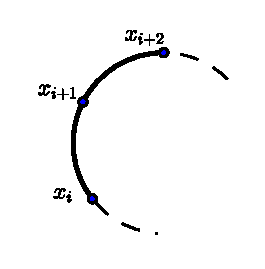
\includegraphics{consecutive_vertices.eps}
		\end{figure}

	\end{column}
\end{columns}

}

\frame{\frametitle{Odd cycles are not 2-colorable}

Using the derivations $\D_1,...,\D_{2n-1}$, we obtain the following derivation of the empty set in $H_{G,2}$:\vspace*{2pt}
$$
\prftree[l]{$x_{2n+1}x_1\in E$}
{ \prftree
{\prftree 
{\prftree{ \prftree{ \prfsummary{\D_1} {\E x_1x_3}  }{  \prfsummary{\D_3}{\E x_3x_5} }
{\E x_1 x_5}}{\prfsummary{ \D_5}{ }}{ \prfsummary{...}{} }{\prfsummary{ \D_{2n-3}}{ }}
{ \E x_1 x_{2n-1}}}{\prfsummary{\D_{2n-1}} { \E x_{2n-1}x_{2n+1}}}
{\E x_1 x_{2n+1} } }  
{\E x_{2n+1}x_1} }
{\emptyset}
$$


}



\frame{ \frametitle{If $G$ has no odd cycles, is 2-colorable }
We prove the equivalent proposition: \\
\textit{"If a graph $G=(V,E)$ is not 2-colorable, then it has an odd cycle"}

\vspace*{2pt}

Every graph that contains $G$ is not 2-colorable; therefore by Robinson's Theorem, we know that  
$$\vdash_{H_{G,2}} \emptyset$$

\vspace*{2pt}


Every tree in  $H_{G,2}$ can be rearranged in such a way that:
\begin{itemize}
\item $\E x_1x_2 \o \E x_2 x_3 \o\E x_1x_3$ are at the \textbl{top}
\item $\E xy \wedge \E yz \rightarrow  \E xz$ are in the  \textbl{middle}
\item $ xy \in E \Rightarrow  \quad  \neg \E xy $ are at the \textbl{bottom}
\end{itemize}


}

\frame{\frametitle{Proof:}
We proceed by \textbl{induction} on the number $k$ of applications of the transitivity rule  $\E xy \wedge \E yz \rightarrow  \E xz$.
If $k=0$ the tree is: 

\vspace*{10pt}
$$
\prftree[l]{$xy \in E$}{
\prftree[l]{$yz \in E$}{
\prftree[l]{$xz \in E$}{
\prftree{ }{ \{ \E xy , \E yz, \E xz  \} } } 
{\{ \E xy , \E yz \} } } 
{ \E xy  } }
{ \emptyset }
$$

\vspace*{10pt}


Then $xy,xz,yz \in E$ and the \textbl{3-cycle} $xyz$ is a subgraph of $G$.
}
\frame{\frametitle{$k>0$}

The tree is of the following form:
$$
\prftree
{\prfsummary[$\D_1$]{\emptyset}{\Gamma_1 \cup \E xy }}
{\prfsummary[$\D_2$]{\emptyset}{\Gamma_2 \cup \E yz }}
{\prfsummary{\Sigma \cup \E xz }{\emptyset}}
$$

For each $\E ab \in \Sigma \cup \E xz  $, we have $ab\in E$, then we have two derivations:
$$
\D'_1:\,\Gamma_1 \vdash_{H_{G,2}} \emptyset \qquad \D'_2:\,\Gamma_1 \vdash_{H_{G,2}} \emptyset
$$
made only of the rule $ ab \in E \Rightarrow   \neg \E ab $ 

}
\frame{\frametitle{$k>0$}
Let $E'=E\cup\{xy,yz\}$ and $G'=(V,E' )$, and consider $H_{G',2}$

\begin{eqnarray*}
\prfsummary[$\D'_1$]{
\prftree[r]{$xy \in E'$}{\prfsummary[$\D_1$]{\emptyset}{\Gamma_1 \cup \E xy}}{\Gamma_1}}
{\emptyset}
&\hspace*{10pt} &
\prfsummary[$\D'_2$]{
\prftree[r]{$yz \in E'$}{\prfsummary[$\D_2$]{\emptyset}{\Gamma_2 \cup\E yz}}{\Gamma_2}}
{\emptyset}
\end{eqnarray*}
By inductive hypothesis, we have \textbl{two odd cycles} in $G'$, say $C_1, C_2$
}

\frame{\frametitle{$k>0$}
\begin{itemize}
\item Say \textit{length}$(C_1)=2n+1$, \textit{length}$(C_2)=2m+1$
\end{itemize}
If $C_1$ and $C_2$ are edge-disjoint
\begin{center}
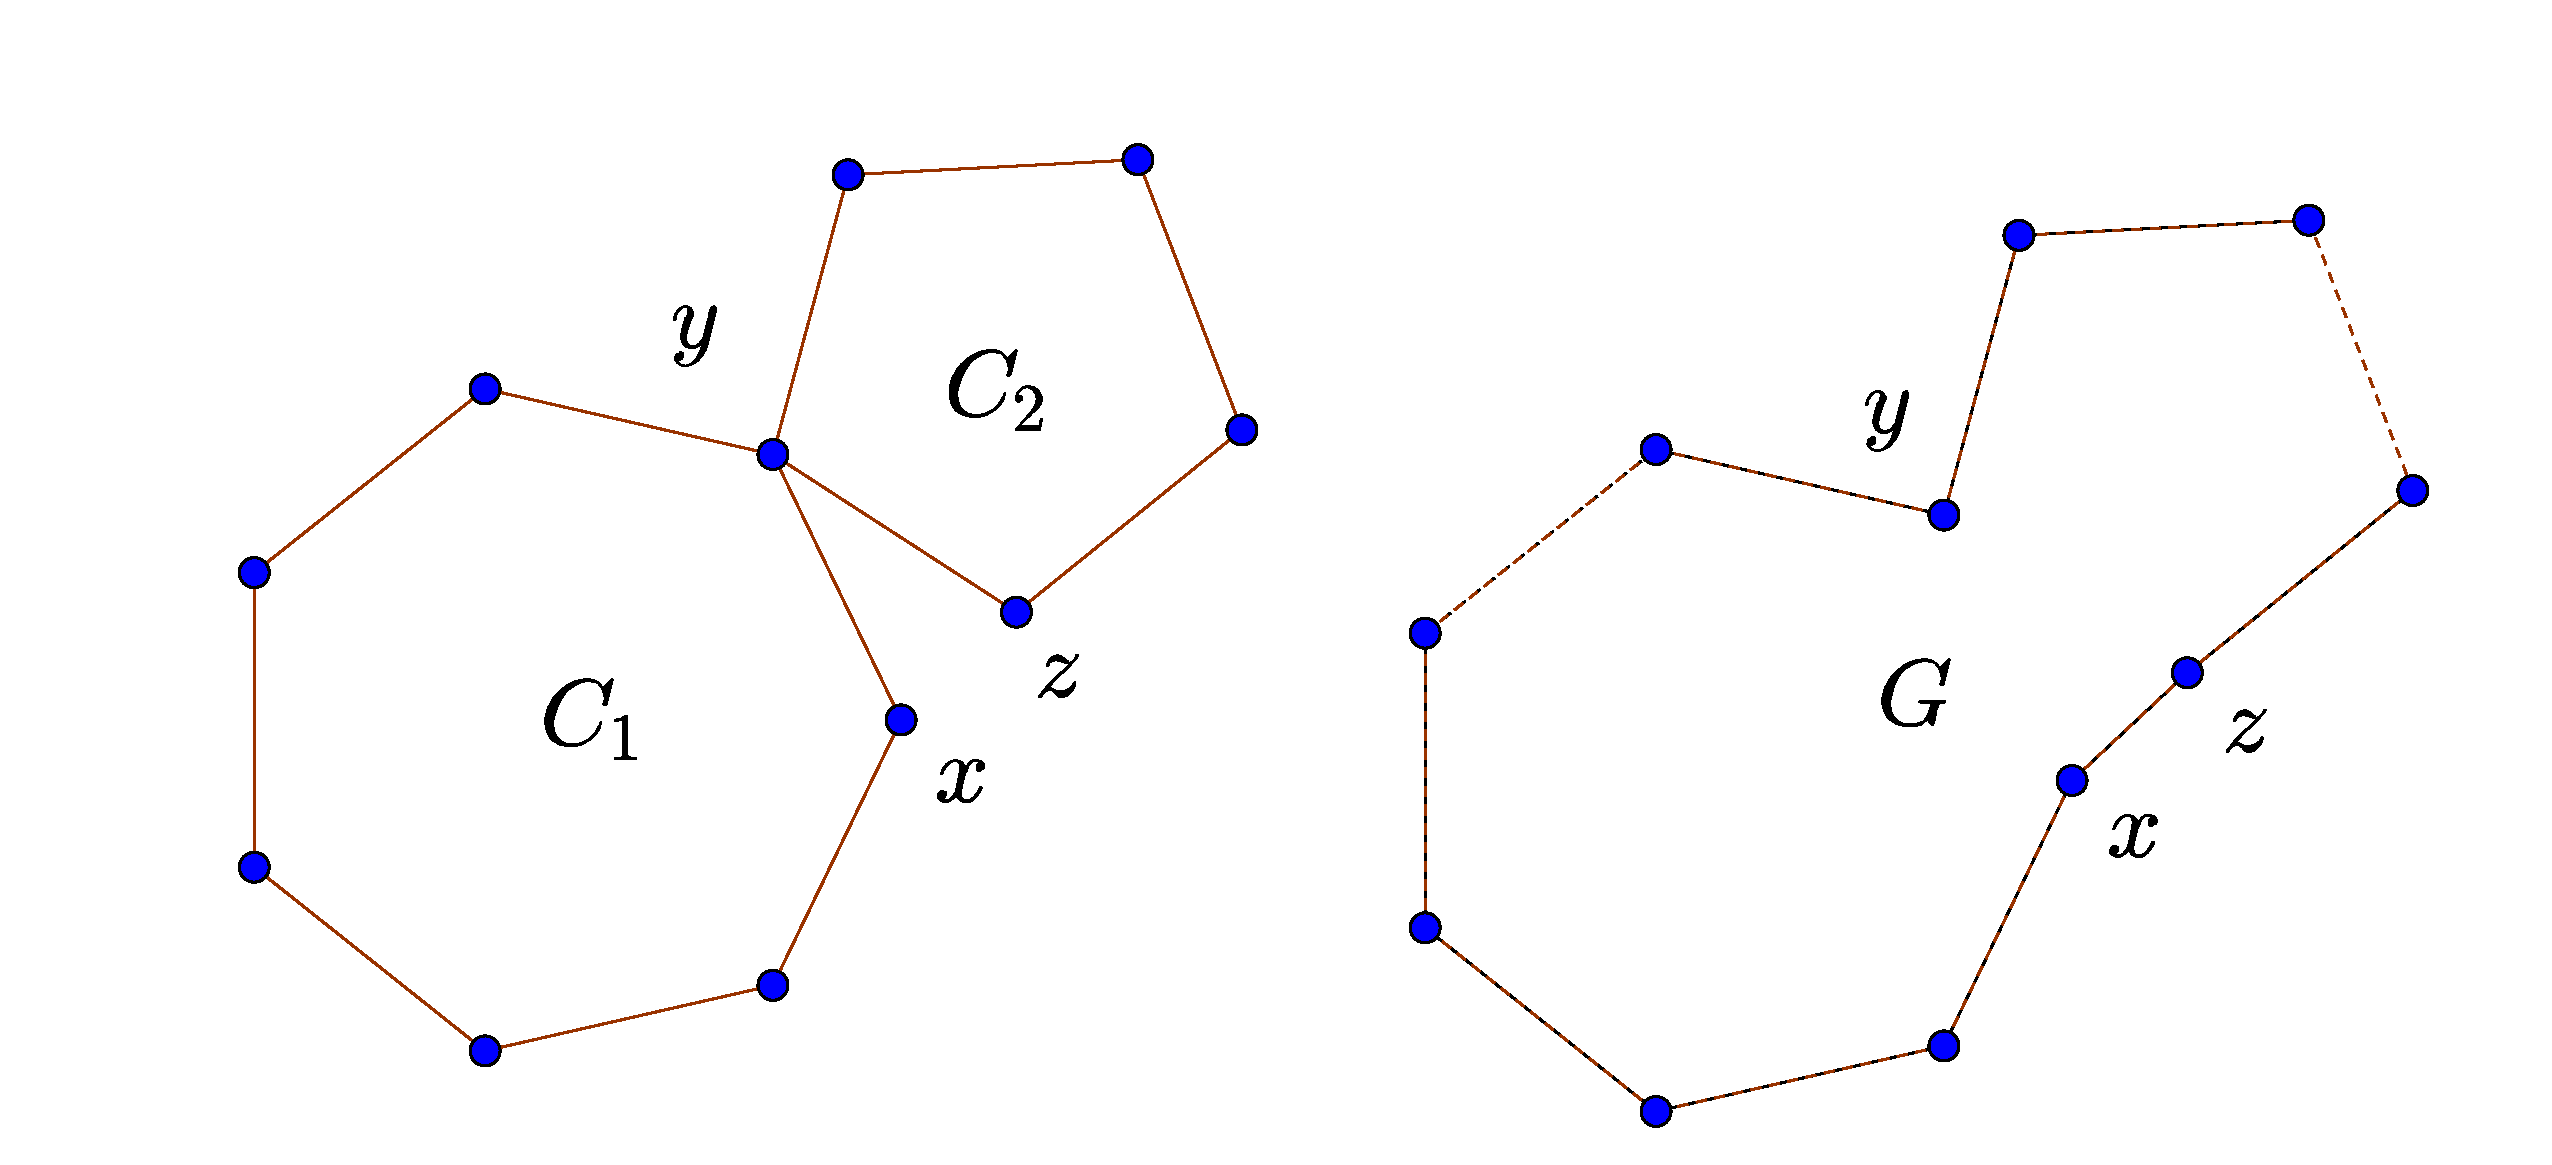
\includegraphics[scale=0.2]{../oddcycles1.eps}
\end{center}
$G$ has a cycle of length $2(n+m)+1$ which is the \textbl{required odd cycle.}

}

\frame{\frametitle{$\mu_n$ graphs}
Inductive definition by by Matijasevi\v{c}: 
\begin{itemize}
\item Every complete graph with $n+1$ vertices is a $\mu_n$-graph
\item If $G_1=(V_1,E_1)$ and $G_2=(V_2,E_2)$ are $\mu_n$-graphs and $a,b,c$ are distinct vertices such that
$$ a,b\in V_1 \quad b,c\in V_2  $$
$$ ab\in E_1, ab\notin E_2 \qquad  bc\in E_2, bc\notin E_1$$
Then the graph $G=(V_1\cup V_2, E_1\cup E_2\cup\{ac\} \setminus\{ab,bc\} )$ is a $\mu_n$-graph.
\end{itemize} 

\begin{theorem}[Matijasevi\v{c}]
\begin{itemize}
\item $\mu_n$ graphs are not $n$-colorable
\item Every graphs which is not $n$-colorable has a $\mu_n$ graph as subgraph.
\end{itemize}
\end{theorem}



}

\frame{\frametitle{$\mu_2$ graphs}

\begin{columns}
	\begin{column}{0.48\textwidth}
		\begin{figure}[htb]
		\includegraphics[scale=0.15]{../triangles.eps}
		\end{figure}
	\end{column}
	\begin{column}{0.48\textwidth}
		\begin{figure}[htb]
		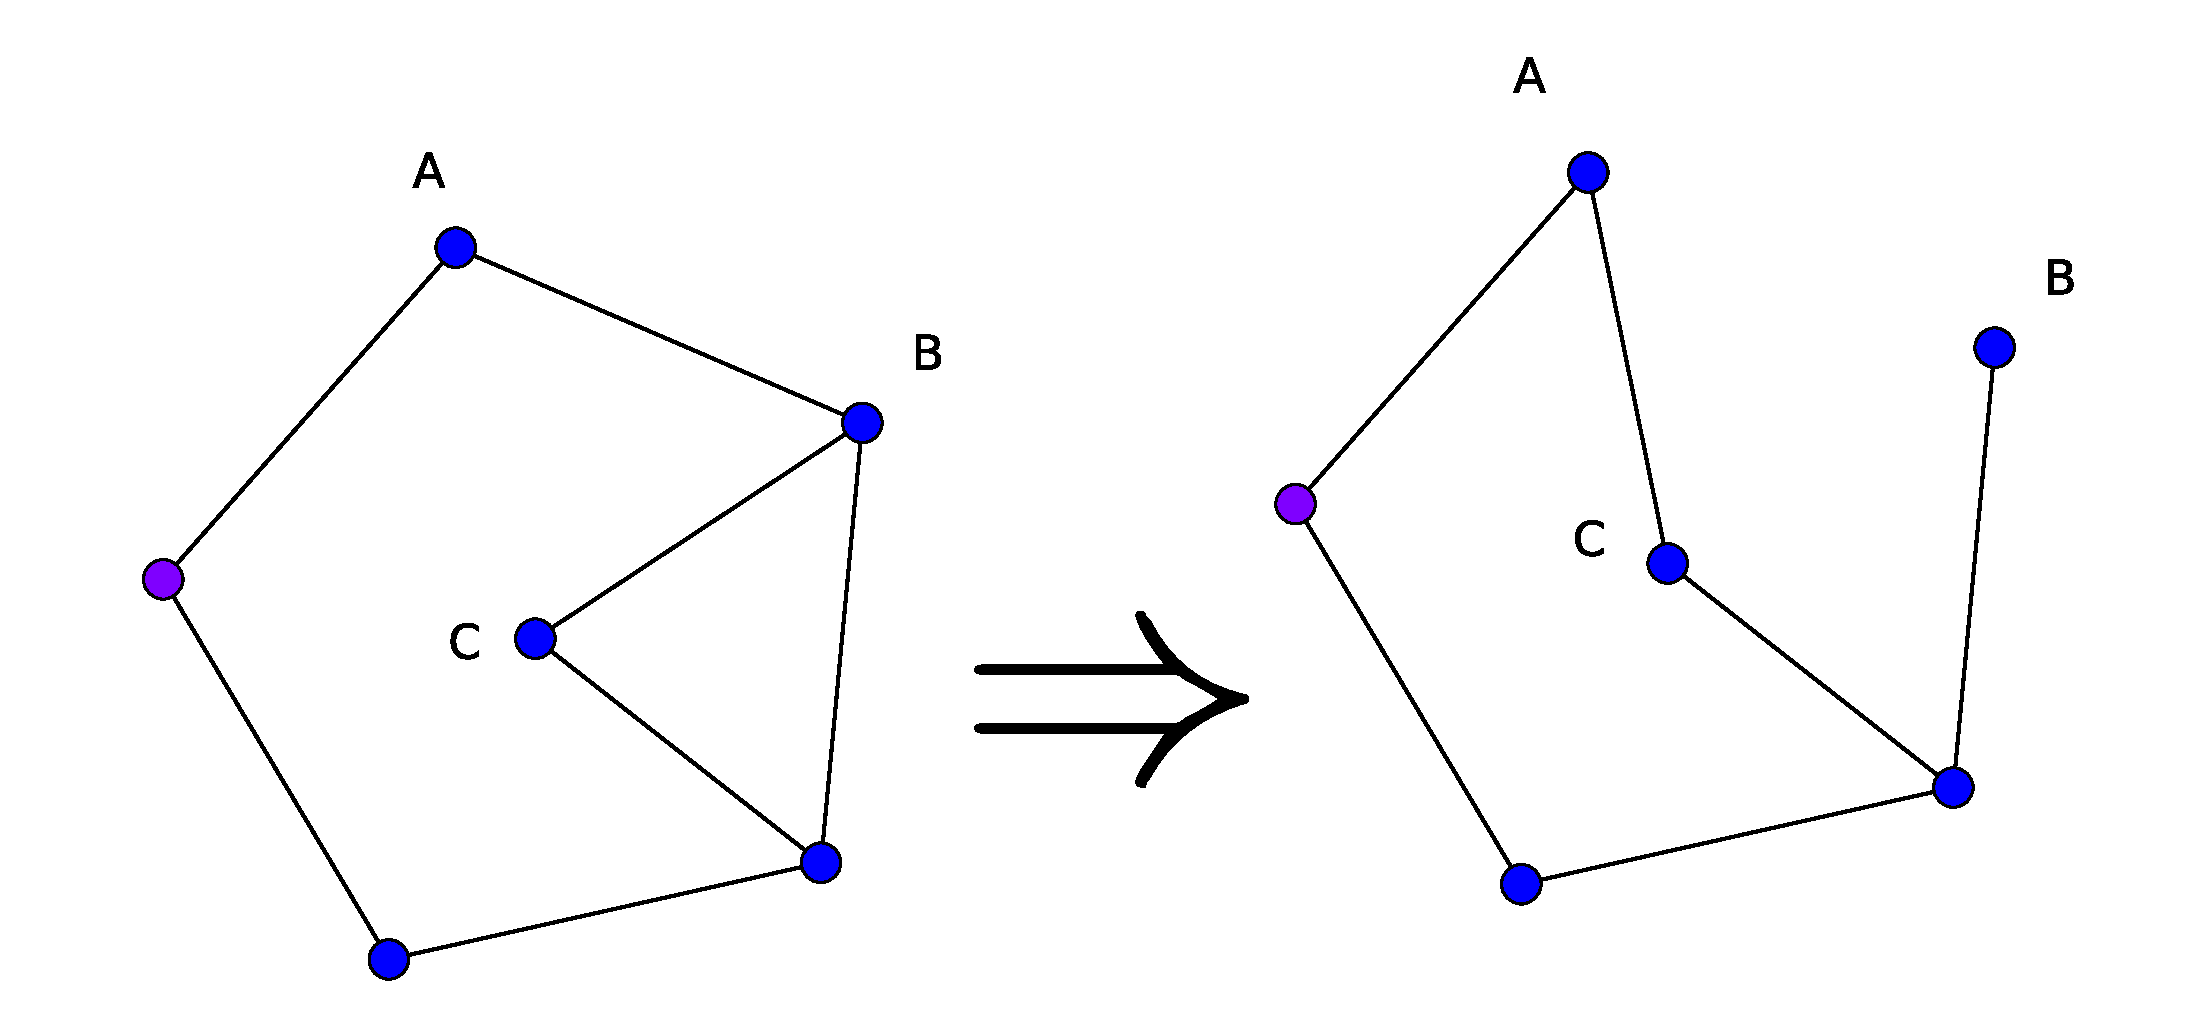
\includegraphics[scale=0.15]{../mu2.eps}
		\end{figure}

	\end{column}
\end{columns}

\begin{figure}[htb]
	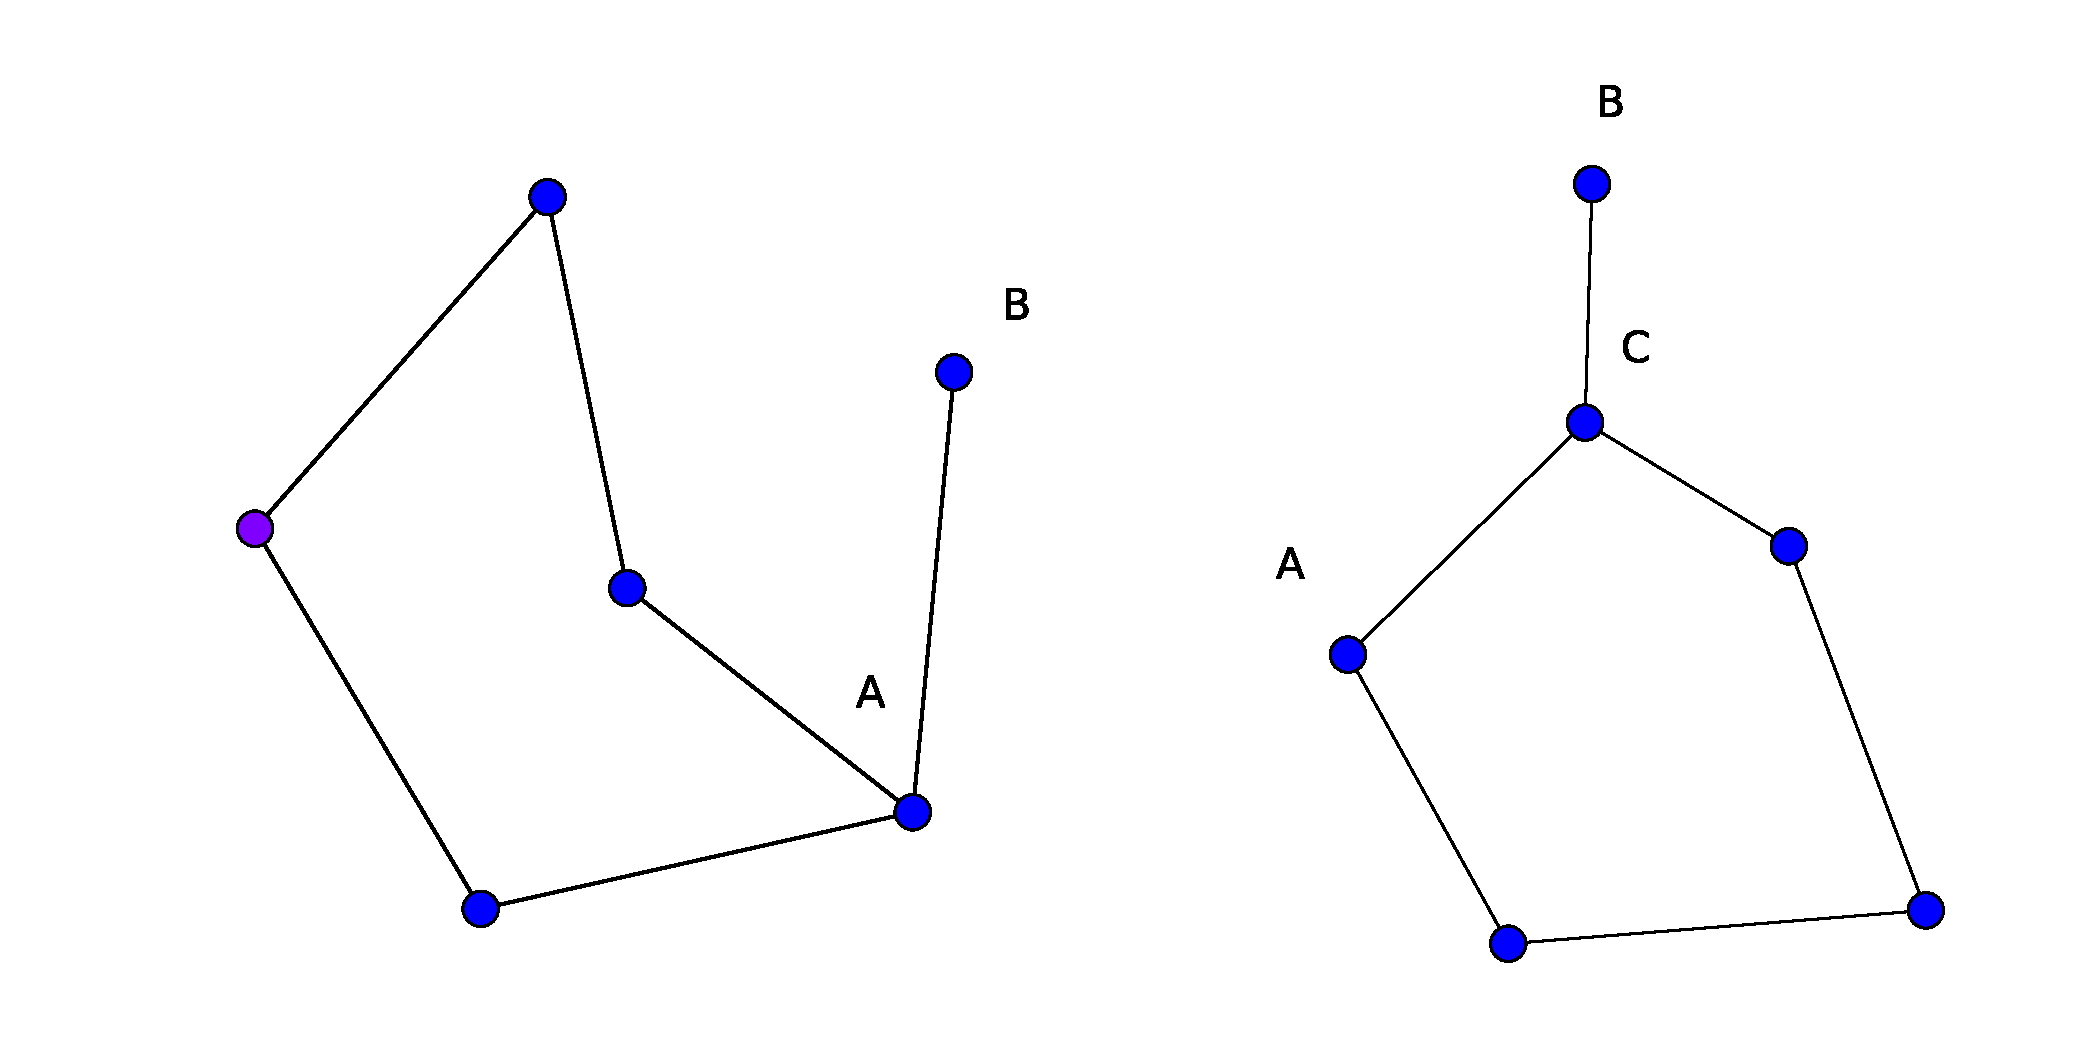
\includegraphics[scale=0.15]{../mu2-con1.eps}
\end{figure}


}


\frame{{Conclusion}
Using Matijasevi\v{c}'s theorem, it is possible to rephrase some problems of graph theory, for instance:

\begin{itemize}
\item \textbl{Four color's theorem: }No $\mu_4$ is planar.
\item \textbl{Hadwiger's conjecture:} Any graph that contains a $\mu_n$ graph has $K^{n+1}$  as minor.

\end{itemize}



\vspace*{50pt}\pausa
\begin{flushright}
\fbox{\huge\textbl{Thank you!}}
\end{flushright}

}

\end{document}



